%-------------------------------------------------------------------------------

%%%%%%%%%%%%%%%%%%%%%%%%%%%%%%%%%%%%%%%%%
% Beamer Presentation
% LaTeX Template
% Version 1.0 (10/11/12)
%
% This template has been downloaded from:
% http://www.LaTeXTemplates.com
%
% License:
% CC BY-NC-SA 3.0 (http://creativecommons.org/licenses/by-nc-sa/3.0/)
%
%%%%%%%%%%%%%%%%%%%%%%%%%%%%%%%%%%%%%%%%%

%-------------------------------------------------------------------------------
%	PACKAGES AND THEMES
%-------------------------------------------------------------------------------

\documentclass{beamer}
\usepackage{xcolor}
\usepackage{graphicx}
\usepackage{tikz}
\usepackage{listings}
\usepackage{multicol}

\definecolor{applegreen}{rgb}{0.55, 0.71, 0.0}
\definecolor{blue(ncs)}{rgb}{0.0, 0.45, 0.60}
\definecolor{burgundy}{rgb}{0.5, 0.0, 0.13}

\definecolor{cadet}{rgb}{0.33, 0.41, 0.47}
\definecolor{airforceblue}{rgb}{0.36, 0.54, 0.66}

\lstdefinestyle{C}{
  language=C,
  emptylines=1,
  breaklines=true,
  basicstyle=\ttfamily\color{black},
  identifierstyle=\ttfamily,
  keywordstyle=\color[rgb]{0.0, 0.0, 1.0},
  stringstyle=\color[rgb]{1.0, 0.0, 0.0},
  commentstyle=\color{gray}\slshape,
}

\lstdefinestyle{assembly}{
  emptylines=1,
  breaklines=true,
  basicstyle=\ttfamily\color{black},
  identifierstyle=\ttfamily,
  keywordstyle=\color[rgb]{1.0, 0.0, 1.0},
  stringstyle=\color[rgb]{1.0, 0.0, 0.0},
  commentstyle=\color{gray}\slshape,
  morekeywords={vmovapd, vfmadd231pd,vfnmadd213pd, vmulpd},
}

\lstdefinestyle{qfunc}{
  language=C,
  emptylines=1,
  breaklines=true,
  basicstyle=\ttfamily\color{black},
  commentstyle=\color{gray}\slshape,
  moredelim=**[is][\color{applegreen}]{@}{@},
  moredelim=**[is][\color{blue(ncs)}]{!}{!},
  moredelim=**[is][\color{green!40!black}]{z}{z},
  moredelim=**[is][\color{blue(ncs)!80}]{#}{#},
  moredelim=**[is][\color{blue(ncs)!80!black}]{'}{'},
}

\lstdefinestyle{oper}{
  language=C,
  emptylines=1,
  breaklines=true,
  basicstyle=\ttfamily\color{black},
  moredelim=**[is][\color{applegreen}]{@}{@},
  moredelim=**[is][\color{blue(ncs)}]{!}{!},
  moredelim=**[is][\color{burgundy}]{#}{#},
  moredelim=**[is][\color{red}]{'}{'},
  moredelim=**[is][\bf]{z}{z},
}

\mode<presentation> {

\usetheme{CambridgeUS}

\usecolortheme{wolverine}

\definecolor{gold}{HTML}{D4A017}
\definecolor{darkgold}{HTML}{B7950B}

\setbeamercolor{palette primary}{bg=cadet,fg=white}
\setbeamercolor{palette secondary}{bg=airforceblue,fg=white}
\setbeamercolor{palette tertiary}{bg=black,fg=white}
\setbeamercolor{palette quaternary}{bg=cadet,fg=white}

\setbeamercolor{frametitle}{bg=airforceblue,fg=white}

\setbeamercolor{section number projected}{bg=black,fg=cadet}
\setbeamercolor{item}{fg=black,bg=cadet}

\setbeamertemplate{page number in head/foot}[framenumber]
}

\usepackage{graphicx} % Allows including images
\usepackage{booktabs} % Allows the use of \toprule, \midrule and \bottomrule in tables

%-------------------------------------------------------------------------------
%	TITLE PAGE
%-------------------------------------------------------------------------------

\title[libCEED Finite Element Library]{Preconditioning with BDDC and FDM\\for High Order Finite Elements with libCEED} % The short title appears at the bottom of every slide, the full title is only on the title page

\author[Jeremy L Thompson]{Jeremy L Thompson\textsuperscript{1}\\
 Valeria Barra\textsuperscript{1}, Yohann Dudouit\textsuperscript{2},
 Oana Marin\textsuperscript{3}, \& Jed Brown\textsuperscript{1}} % Your name
\institute[CU Boulder] % Your institution as it will appear on the bottom of every slide, may be shorthand to save space
{1: University of Colorado Boulder \\
 2: Lawrence Livermore National Laboratory \\
 3: Argonne National Laboratory \\ % Your institution for the title page
\medskip
\textit{jeremy.thompson@colorado.edu} % Your email address
}
\date{Jan 15, 2020} % Date, can be changed to a custom date

\begin{document}

\begin{frame}
\titlepage % Print the title page as the first slide
\end{frame}

%-------------------------------------------------------------------------------

\begin{frame}
\begin{center}
\frametitle{libCEED Team}

{\flushleft

Developers: \hspace{2mm} Jed Brown\textsuperscript{1}, Jeremy Thompson\textsuperscript{1} \\
\hspace{23mm}  Thilina Rathnayake\textsuperscript{4}, Jean-Sylvain Camier\textsuperscript{2}, Tzanio Kolev\textsuperscript{2},\\
\hspace{23mm} Veselin Dobrev\textsuperscript{2}, Valeria Barra\textsuperscript{1}, Yohann Doudouit\textsuperscript{2},\\
\hspace{23mm} David Medina\textsuperscript{5}, Tim Warburton\textsuperscript{6}, \& Oana Marin\textsuperscript{3}\\

~\\

Grant: \hspace{11mm} Exascale Computing Project (17-SC-20-SC)\\

~\\

~\\

\small{1: University of Colorado, Boulder\\
2: Lawrence Livermore National Laboratory\\
3: Argonne National Laboratory\\
4: University of Illinois, Urbana-Champaign\\
5: OCCA\\
6: Virginia Polytechnic Institute and State University\\}}

\end{center}
\end{frame}

%-------------------------------------------------------------------------------

\begin{frame}
\begin{center}
\frametitle{Overview}

High order matrix-free finite elements are less expensive than\\
sparse matrices, with respect to both FLOPS and memory transfer\\

~\\

~\\

libCEED's finite element operator decomposition provides performance,\\
portability, and opportunities for flexible preconditioning strategies\\

~\\

~\\

Fast Diagonalization Method compliments the libCEED decomposition and\\
provides inexact subdomain solvers for BDDC or ASM preconditioning

\end{center}
\end{frame}
 
%-------------------------------------------------------------------------------

\begin{frame}
\frametitle{Overview} % Table of contents slide, comment this block out to remove it
\tableofcontents
\end{frame}

%-------------------------------------------------------------------------------
%	PRESENTATION SLIDES
%-------------------------------------------------------------------------------

%-------------------------------------------------------------------------------
\section{Introduction}
%-------------------------------------------------------------------------------

\begin{frame}
\begin{center}
\frametitle{Center for Efficient Exascale Discretizations}

\begin{flushleft}
DoE exascale co-design center\\

~\\
\end{flushleft}

\begin{itemize}

\item Design discretization algorithms for exascale hardware that deliver significant performance gain over low order methods\\

~\\

\item Collaborate with hardware vendors and software projects for exascale hardware and software stack\\

~\\

\item Provide efficient and user-friendly unstructured PDE discretization component for exascale software ecosystem

\end{itemize}

\end{center}
\end{frame}

%-------------------------------------------------------------------------------

\begin{frame}
\begin{center}
\frametitle{FLOPs vs Bandwidth}

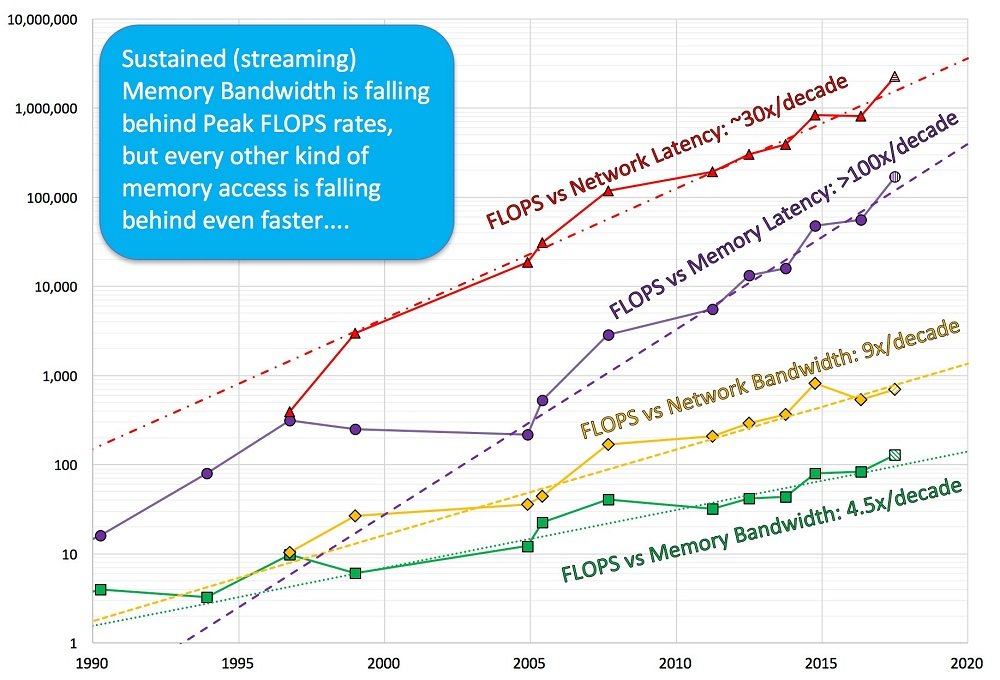
\includegraphics[height=6.5cm]{McCalpinFLOPsVsBandwidth}

Growth of FLOPs outstriping bandwidth for decades, McCalpin SC16

\end{center}
\end{frame}

%-------------------------------------------------------------------------------

\begin{frame}
\begin{center}
\frametitle{Tensor Product Elements}

\setlength{\columnsep}{15mm}
\begin{multicols}{2}

\begin{flushright}
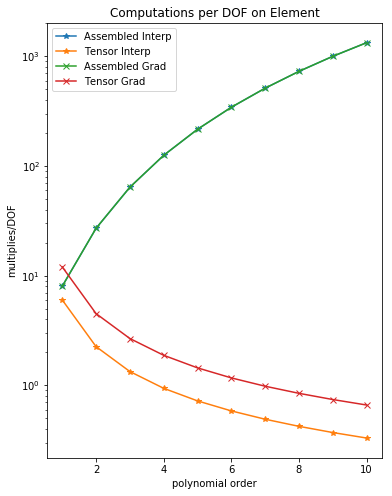
\includegraphics[height=5cm]{libCEEDAssembledVsTensorApply}
\end{flushright}

\begin{flushleft}
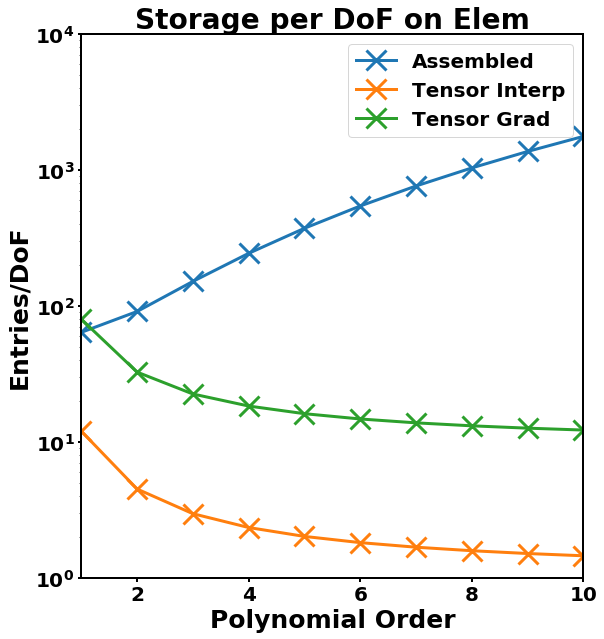
\includegraphics[height=5cm]{libCEEDAssembledVsTensorStorage}
\end{flushleft}

\end{multicols}

Matrix-free finite element formulations provide performance\\
optimizations for hexahedral elements

\end{center}
\end{frame}

%-------------------------------------------------------------------------------
\section{libCEED}
%-------------------------------------------------------------------------------

\begin{frame}
\begin{center}
\frametitle{libCEED Operator Decomposition}

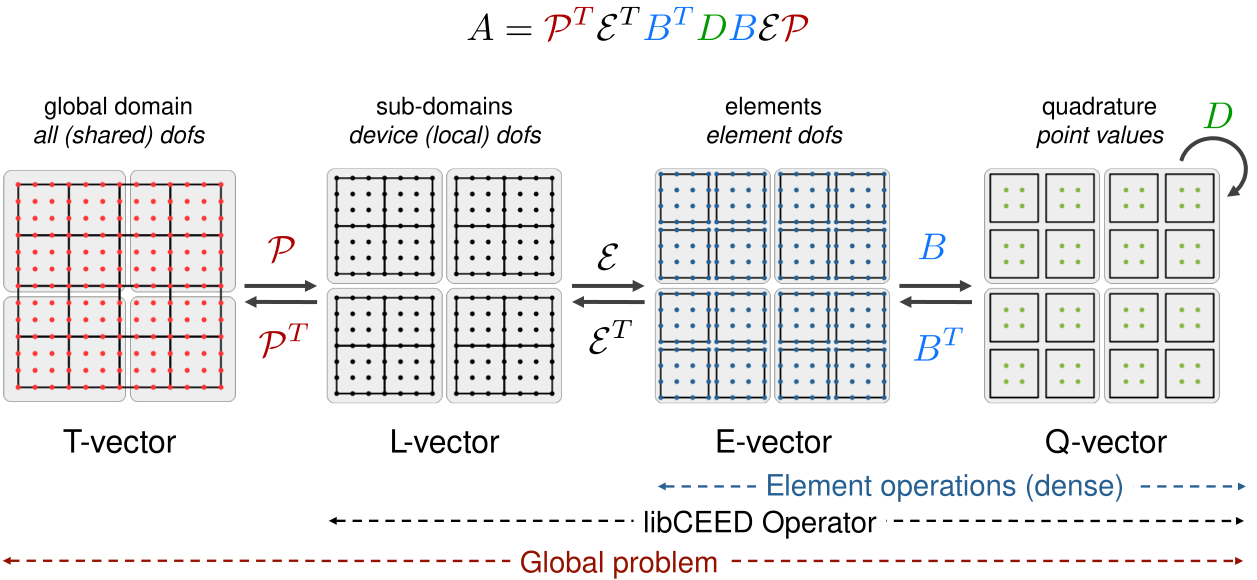
\includegraphics[height=4.7cm]{libCEEDAPI}

\small{

\hspace{1.8cm}${\color{burgundy}A}_L = G^T {\color{blue(ncs)}B^T} {\color{applegreen}D} {\color{blue(ncs)}B} G$

\begin{itemize}

\item $G$ - CeedElemRestriction, local gather/scatter

\item {\color{blue(ncs)}$B$} - CeedBasis, provides basis operations such as interp and grad

\item {\color{applegreen}$D$} - CeedQFunction, representation of PDE at quadrature points

\item ${\color{burgundy}A}_L$ - CeedOperator, aggregation of Ceed objects for local action of operator

\end{itemize}

}

\end{center}
\end{frame}

%-------------------------------------------------------------------------------

\begin{frame}
\begin{center}
\frametitle{Laplacian Example}

Solving the 2D Poisson problem: $-\Delta u = f$\\

Weak Form: $\int \nabla v \nabla u = \int v f$\\
~\\

\begin{itemize}

\item General libCEED Operator

      ${\color{burgundy}A}_L = G^T {\color{blue(ncs)}B^T} {\color{applegreen}D} {\color{blue(ncs)}B} G$\\
~\\

\item Laplacian Operator

      ${\color{burgundy}A}_L = G^T {\color{blue(ncs)} \nabla B^T} {\color{applegreen}D} {\color{blue(ncs)} \nabla B} G$

\end{itemize}

where ${\color{applegreen}D}$ is block diagonal by quadrature point:\\
      ${\color{applegreen}D_i} = J_{geo}^{-1} \left( w_i \det{J_{geo}}\right) J_{geo}^{-T}$ and
      $J_{geo} = \left[ \begin{tabular}{cc}
$\frac{\partial x}{\partial r}$ & $\frac{\partial x}{\partial s}$\\
$\frac{\partial y}{\partial r}$ & $\frac{\partial y}{\partial s}$
\end{tabular} \right]$\\
      $x, y$ physical coords; $r, s$ reference coords

\end{center}
\end{frame}

%-------------------------------------------------------------------------------

\begin{frame}
\begin{center}
\frametitle{Helmholtz Example}

Solving the 2D Inhomogeneous Helmholtz problem: $-\left( \Delta + k^2 \right) u = f$\\

Weak Form: $\int \left( \nabla v \nabla u - k^2 v u \right) = \int v f$\\
~\\

\begin{itemize}

\item General libCEED Operator

      ${\color{burgundy}A}_L = G^T {\color{blue(ncs)}B^T} {\color{applegreen}D} {\color{blue(ncs)}B} G$\\
~\\

\item Helmholtz Operator

      ${\color{burgundy}A}_L = G^T \left[ \begin{array}{c} {\color{blue(ncs)}B} \\ {\color{blue(ncs)}\nabla B} \end{array} \right]^T {\color{applegreen}D} \left[ \begin{array}{c} {\color{blue(ncs)}B} \\ {\color{blue(ncs)}\nabla B} \end{array} \right] G$

\end{itemize}

where ${\color{applegreen}D}$ is block diagonal by quadrature point:\\
      ${\color{applegreen}D_i} = \left( w_i \det{J_{geo}}\right) \left[ \begin{array}{c c} -k^2 \\ & J_{geo}^{-1} J_{geo}^{-T} \end{array} \right]$ and
      $J_{geo} = \left[ \begin{tabular}{cc}
$\frac{\partial x}{\partial r}$ & $\frac{\partial x}{\partial s}$\\
$\frac{\partial y}{\partial r}$ & $\frac{\partial y}{\partial s}$
\end{tabular} \right]$\\
      $x, y$ physical coords; $r, s$ reference coords

\end{center}
\end{frame}

%-------------------------------------------------------------------------------

\iffalse

\begin{frame}[fragile]
\begin{center}
\frametitle{Operator Definition}

General libCEED Operator:\\

${\color{red}v}_L = {\color{burgundy}A}_L {\color{red}u}_L$\\

~\\

${\color{burgundy}A}_L = G^T {\color{blue(ncs)}B^T} {\color{applegreen}D} {\color{blue(ncs)}B} G$\\

~\\~\\

Laplacian Operator Code:
{\scriptsize
\begin{lstlisting}[style=oper]
CeedOperatorCreate(ceed, @qf_apply@, NULL, NULL, &#op_apply#);
CeedOperatorSetField(#op_apply#, "du", zerestrictuz, CEED_TRANSPOSE,
                     !basisu!, 'CEED_VECTOR_ACTIVE');
CeedOperatorSetField(#op_apply#, "geo",erestrictqdi,CEED_NOTRANSPOSE,
                     !CEED_BASIS_COLLOCATED!, geo);
CeedOperatorSetField(#op_apply#, "dv", zerestrictuz, CEED_TRANSPOSE,
                     !basisu!, 'CEED_VECTOR_ACTIVE');
...
CeedOperatorApply(#op_apply#, 'uloc', 'vloc', CEED_REQUEST_IMMEDIATE);
\end{lstlisting}
}

\end{center}
\end{frame}

%-------------------------------------------------------------------------------

\begin{frame}[fragile]
\begin{center}
\frametitle{QFunction Definition}

General libCEED QFunction:\\

${\color{blue(ncs)!80!black}v_q} = {\color{applegreen}D} {\color{blue(ncs)!80}u_q}$\\

~\\

2D Laplacian QFunction:\\

${\color{blue(ncs)}\left[} {\color{blue(ncs)!80!black} \begin{tabular}{c}
$dv_0$\\ $dv_1$ \end{tabular}} {\color{blue(ncs)}\right]} = {\color{applegreen} \left[} {\color{green!40!black} \begin{tabular}{cc}
$D_{00}$ & $D_{01}$\\
$D_{01}$ & $ D_{11}$ \end{tabular}} {\color{applegreen}\right]} {\color{blue(ncs)}\left[} {\color{blue(ncs)!80} \begin{tabular}{c}
$du_0$\\ $du_1$ \end{tabular} } {\color{blue(ncs)}\right]}$\\

~\\

~\\

2D Laplacian QFunction Code:
{\scriptsize
\begin{lstlisting}[style=qfunc]
CeedQFunctionCreateInterior(ceed, 1, Poisson2D,
                            Poisson2D_loc, &@qf_apply@);
CeedQFunctionAddInput(@qf_apply@, #"du"#, 2, !CEED_EVAL_GRAD!);
CeedQFunctionAddInput(@qf_apply@, z"geo"z, 3, CEED_EVAL_NONE);
CeedQFunctionAddOutput(@qf_apply@, '"dv"', 2, !CEED_EVAL_GRAD!);
\end{lstlisting}
}

\end{center}
\end{frame}

%-------------------------------------------------------------------------------

\begin{frame}[fragile]
\begin{center}
\frametitle{QFunction Definition}

\begin{itemize}

\item Single Source QFunctions for all backends:\\

~\\

\item C/C++ code, compiled with main for CPU, JiT for GPU\\

\end{itemize}

~\\

{\scriptsize
\begin{lstlisting}[style=qfunc]
int Poisson2D(void *ctx, const CeedInt Q,
    const CeedScalar *const *in, CeedScalar *const *out) {
  // Inputs and Outputs
  const CeedScalar #*du# = in[0];
  CeedScalar z*geoz = out[0], '*dv' = out[1];

  // Quadrature Point Loop
  CeedPragmaSIMD // For CPU vectorization
  for (CeedInt i=0; i<Q; i++) {
    'dv[i+Q*0]' = zgeo[i+Q*0]z*#du[i+Q*0]# + zgeo[i+Q*2]z*#du[i+Q*1]#;
    'dv[i+Q*1]' = zgeo[i+Q*2]z*#du[i+Q*0]# + zgeo[i+Q*1]z*#du[i+Q*1]#;
  } // End of Quadrature Point Loop

  return 0;
}
\end{lstlisting}
}

\end{center}
\end{frame}

\fi

%-------------------------------------------------------------------------------
\section{Preconditioning Methods}
%-------------------------------------------------------------------------------

\begin{frame}
\begin{center}
\frametitle{Domain Decomposition Preconditioning}

\begin{itemize}

\item Preconditioning essential for iterative solvers, especially with high
order elements\\

~\\

\item P-Multigrid preconditioning offers $O(N)$ elliptic PDE solve\\

\begin{itemize}

\item Requires careful communication implementation for parallel performance

\end{itemize}

~\\

\item Additive Schwartz with high order element subdomains

\begin{itemize}

\item Element halo can be large and complicated in unstructured meshes

\end{itemize}

~\\

\item BDDC/FETI eliminate the halo, needs unassembled operator

\begin{itemize}

\item Requires subdomain continuity conditions to converge

\end{itemize}

\end{itemize}

\end{center}
\end{frame}

%-------------------------------------------------------------------------------

\begin{frame}
\begin{center}
\frametitle{Additive Schwartz}

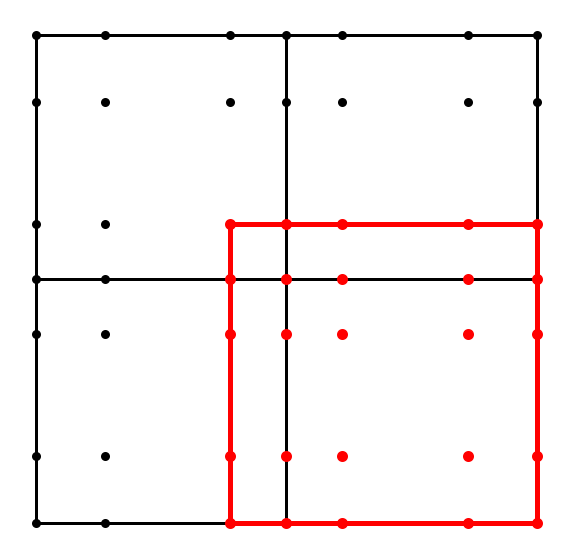
\includegraphics[height=4.7cm]{libCEEDASM}

\begin{itemize}

\item Tradeoff with overlap in convergence and computations/bandwidth\\

~\\

\item See Nek5000 pressure solves, work by Fischer, Miller, and Tufo

\end{itemize}

\end{center}
\end{frame}

%-------------------------------------------------------------------------------

\begin{frame}
\begin{center}
\frametitle{BDDC}

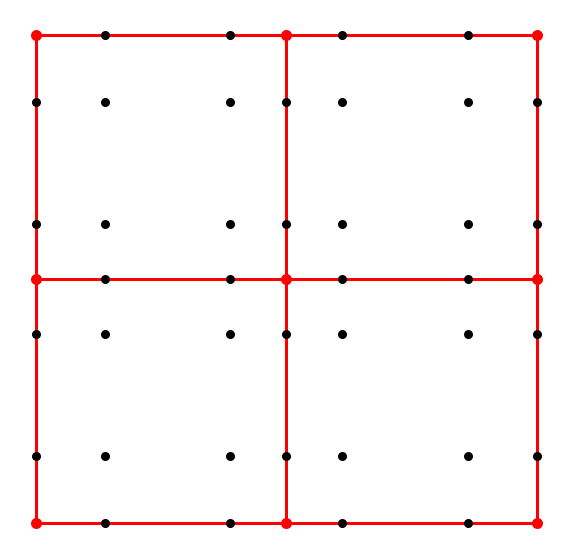
\includegraphics[height=4.7cm]{libCEEDBDDC}

\begin{itemize}

\item Global coarse solve gives boundary conditions for subdomain solves\\

~\\

\item See BDDC preconditioner in PETSc, work by Zampini

\end{itemize}

\end{center}
\end{frame}

%-------------------------------------------------------------------------------
\section{Subdomain Solvers}
%-------------------------------------------------------------------------------

\begin{frame}
\begin{center}
\frametitle{Inexact Subdomain Solves}

\begin{itemize}

\item Li and Widlund 2007 demonstrated BDDC with inexact subdomain solves using multigrid\\

~\\

\item Fast Diagonalization provides inverses of separable operators\\

\begin{itemize}

\item Used in Nek5000 with Additive Schwartz subdomain solves

\end{itemize}

~\\

\item Fast Diagonalization can provide inexact subdomain solves for BDDC\\

\begin{itemize}

\item Open question: Which non-separable operators can use FDM based inexact subdomain solves?

\end{itemize}

\end{itemize}

\end{center}
\end{frame}

%-------------------------------------------------------------------------------

\begin{frame}
\begin{center}
\frametitle{Fast Diagonalization Method}

\begin{itemize}

\item Consider 2D Helmholtz problem on a reference element\\

\begin{center}

~\\

Let $A = \nabla B^T w \nabla B$, $M = B^T w B$\\

~\\

$L = A_{2D} - k^2 M_{2D} = A \otimes A - k^2 M \otimes M$

\end{center}

~\\

\item Diagonalize 1D element Laplacian and mass matrix\\

~\\

\begin{center}

$P^T A P = \Lambda$, $P^T M P = I$

\end{center}

~\\

\item Build element inverse

~\\

\begin{center}

$L^{-1} = P \otimes P \left[ \Lambda \otimes I + I \otimes \Lambda - k^2 I \otimes I \right]^{-1} P^T \otimes P^T$

\end{center}

~\\

\end{itemize}

\end{center}
\end{frame}

%-------------------------------------------------------------------------------

\begin{frame}
\begin{center}
\frametitle{Inverse of Separable Operators}

\begin{itemize}

\item In general\\

~\\

\begin{center}

$L = c A_{2D} + k M_{2D} = c \left( A_x \otimes A_y \right) + k \left( M_x \otimes M_y \left)$

\end{center}

~\\

\item Diagonalize 1D element Laplacians and mass matrices\\

~\\

\begin{center}

$P^T A_x P = \chi \Lambda$, $P^T M_x P = \chi I$\\
$P^T A_y P = \Lambda$, $P^T M_y P = I$

\end{center}

~\\

\item Build element inverse

~\\

\begin{center}

$L^{-1} = P \otimes P \left[ c \left( \chi \Lambda \otimes I \right) + c \left( \chi I \otimes \Lambda \right) + k \left( \chi I \otimes I \right) \right]^{-1} P^T \otimes P^T$

\end{center}

~\\

\end{itemize}

\end{center}
\end{frame}

%-------------------------------------------------------------------------------

\begin{frame}
\begin{center}
\frametitle{Nonlinear Coefficients}

\begin{itemize}

\item Generalized inhomogeneous Helmholtz equation\\

~\\

\begin{center}

$- \left( f_1 \left( x \right) \Delta u + k^2 f_0 \left( x \right) u \right) = f$

\end{center}

~\\

\item Discretized generalized inhomogeneous Helmholtz operator\\

~\\

\end{itemize}

${\color{burgundy}A}_e = \left[ \begin{array}{c} {\color{blue(ncs)}B} \\ {\color{blue(ncs)}\nabla B} \end{array} \right]^T {\color{applegreen}D} \left[ \begin{array}{c} {\color{blue(ncs)}B} \\ {\color{blue(ncs)}\nabla B} \end{array} \right]$\\


~\\

where ${\color{applegreen}D_i} = \left( w_i \det{J_{geo}}\right) \left[ \begin{array}{c c} -k^2 f_0 \left( x \right) \\ & J_{geo}^{-1} f_1 \left( x \right) J_{geo}^{-T} \end{array} \right]$\\

~\\

\begin{itemize}

\item Approximate element inverse

~\\

\begin{center}

${\color{burgundy}A}_e^{-1} \approx P \otimes P \left( \Lambda_g \right)^{-1} P^T \otimes P^T$\\
where $\Lambda_g = diag \left( P^T \otimes P^T \left( {\color{burgundy}A}_e \right) P \otimes P \right)$

\end{center}

~\\

\end{itemize}

\end{center}
\end{frame}

%-------------------------------------------------------------------------------

\begin{frame}
\begin{center}
\frametitle{Separable Approximate Inverses}

\begin{itemize}

\item Weak form of general second order PDE\\

~\\

\begin{center}

$\int \left( \nabla v f_1 \left( \nabla u, u, x \right) + v f_0 \left( \nabla u, u, x \right) \right) = \int v f$

\end{center}

~\\

\item Discretized generalized inhomogeneous Helmholtz operator\\

~\\

\end{itemize}

${\color{burgundy}A}_e = \left[ \begin{array}{c} {\color{blue(ncs)}B} \\ {\color{blue(ncs)}\nabla B} \end{array} \right]^T {\color{applegreen}D} \left[ \begin{array}{c} {\color{blue(ncs)}B} \\ {\color{blue(ncs)}\nabla B} \end{array} \right]$\\


~\\

where ${\color{applegreen}D_i} = \left[ \begin{array}{c c} I \\ & J_{geo}^{-1} \end{array} \right] \left( w_i \det{J_{geo}}\right) \left[ \begin{array}{c c} f_{0, 0} & f_{0, 1} \\ f_{1, 0} & f_{1, 1} \end{array} \right] \left[ \begin{array}{c c} I \\ & J_{geo}^{-T} \end{array} \right]$\\

~\\

\begin{itemize}

\item Approximate element inverse

~\\

\begin{center}

${\color{burgundy}A}_e^{-1} \approx ???$

\end{center}

~\\

\end{itemize}


\end{center}
\end{frame}

%-------------------------------------------------------------------------------
\section{Future Work}
%-------------------------------------------------------------------------------

\begin{frame}
\begin{center}
\frametitle{Future Work}

\begin{itemize}

\item Further performance enhancements (GPU and CPU)\\

~\\

\item Improved mixed mesh and operator composition support\\

~\\

\item Expanded non-linear and multi-physics examples\\

~\\

\item Preconditioning based on libCEED operator decomposition\\

~\\

\item Algorithmic differentiation of user quadrature functions\\

~\\

\item We invite contributors and friendly users

\end{itemize}

\end{center}
\end{frame}

%-------------------------------------------------------------------------------
\section{Questions}
%-------------------------------------------------------------------------------

\begin{frame}
\begin{center}
\frametitle{Questions?}

{\flushleft

Advisors : \hspace{5mm} Jed Brown\textsuperscript{1} \& Daniel Appel\"{o}\textsuperscript{1}\\

~\\

Collaborators: Valeria Barra\textsuperscript{1}, Oana Marin\textsuperscript{2}, Tzanio Kolev\textsuperscript{3},\\
\hspace{23mm} Jean-Sylvain Camier\textsuperscript{3}, Veselin Dobrev\textsuperscript{3}, Yohann Doudouit\textsuperscript{3},\\
\hspace{23mm} Tim Warburton\textsuperscript{4}, David Medina\textsuperscript{5}, \& Thilina Rathnayake\textsuperscript{6}\\

~\\

Grant: \hspace{11mm} Exascale Computing Project (17-SC-20-SC)\\

~\\

~\\

\small{1: University of Colorado, Boulder\\
2: Argonne National Laboratory\\
3: Lawrence Livermore National Laboratory\\
4: Virginia Polytechnic Institute and State University\\
5: OCCA\\
6: University of Illinois, Urbana-Champaign\\}}

\end{center}
\end{frame}

%-------------------------------------------------------------------------------

\begin{frame}
\titlepage % Print the title page
\end{frame}

%-------------------------------------------------------------------------------
\end{document}
%-------------------------------------------------------------------------------
